This mini module is an introduction to the principal of \textit{Cognitive Radio}. The idea behind the concept is to distribute  the access to the medium/spectrum in a dynamic way. \\

\textit{From Wikipedia, the free encyclopedia}\\
A cognitive radio is an intelligent radio that can be programmed and configured dynamically. Its transceiver is designed to use the best wireless channels in its vicinity. Such a radio automatically detects available channels in wireless spectrum, then accordingly changes its transmission or reception parameters to allow more concurrent wireless communications in a given spectrum band at one location. This process is a form of dynamic spectrum management.

\section{Choice of Sharing Strategy}
In order to be able to access the spectrum in a dynamic way different strategies can be used one of them is simply to divide the spectrum in a way according to the changing need from the different users. This could either be in time or frequency. The problem in doing this is that you do not utilize the complete spectrum for the different users giving that efficiency is lost.\\

As an example can be used \figref{fig:TimeSlots} where there is unused time in between bursts of transmission, these could be used by a secondary system.  
\begin{figure}[!h]
  \centering
  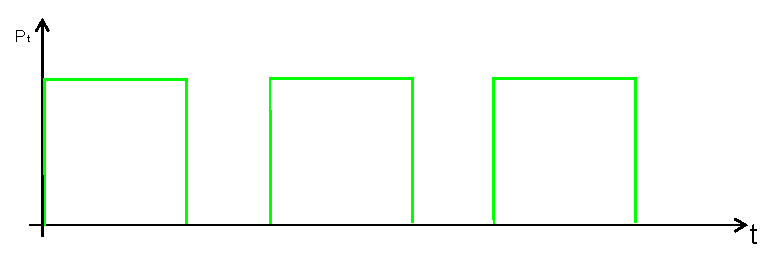
\includegraphics[width=8cm]{TimeSlots.eps}
  \caption{Spectrum use over time}
  \label{fig:TimeSlots}
\end{figure}

However this is as mentioned not the best way of managing the spectrum as the burst of transmission from the primary transmitter could not be periodic or in varying length. If this is the case and the secondary transmitter transmit while the primary transmitter is also transmitting then interference will occur. Due to this a balance of what interference can be allowed have to be made. 